\documentclass[12pt, letterpaper]{article}
\usepackage[english]{babel}
\usepackage[utf8]{inputenc}
\usepackage[T1]{fontenc}
\usepackage{float}
\usepackage[top=0.7cm, bottom=2.0cm, outer=2.0cm, inner=2.0cm, margin=2.0cm]{geometry}
\usepackage{graphicx}
\graphicspath{ {./images/} }
\usepackage{hyperref}
\title{ CS 440: Introduction to AI - Homework 1}
\author{Bhavya Patel (RUID: 200009834), \\Atharva Patil (RUID: 200002655), \\Akshat Mehta (RUID: 201001968)}
\date{February 21, 2023}
\begin{document}
\maketitle

\textbf{NOTE: The statistics presented in this lab report use the built-in Python heapq library as it is more efficient than our own Heap class and thus provides slightly better runtimes. Forward, Backward, and Adaptive A* all still work with our own Heap class, as we will show in the demo, but the runtimes are just slightly slower.}
\\
\section*{Part 0}
Our program uses an algorithm from \textbf{\href{https://edtg.co.uk/2020/04/16/procedural-maze-generator-using-python/}{Online Maze Generator}} to randomly generate the 101 x 101 mazes as 2D arrays of 1s (open cells) and 0s (obstacles). The algorithm we are using for this part is based on Prim’s algorithm, and it guarantees that every maze it generates will have a path from the cell in the top-left corner (0, 0) to the bottom-right (100, 100). In most cases, multiple valid paths will exist. We then feed this maze to our Repeated Forward A*, Repeated Backward A*, and Adaptive A* algorithms. We provide the option to visualize the initial maze, as well as the path generated by the search algorithm from the initial state to the goal state. We only show the path actually traveled by the agent in our visualization, but it is possible to also display the complete path suggested by each A* call in the terminal. Figures are provided below to show the visualizations we generated. White cells can be traversed, gray cells represent obstacles, green cells represent the initial and goal cells, and blue cells represent the path traversed by the agent.

\begin{figure}
\centering
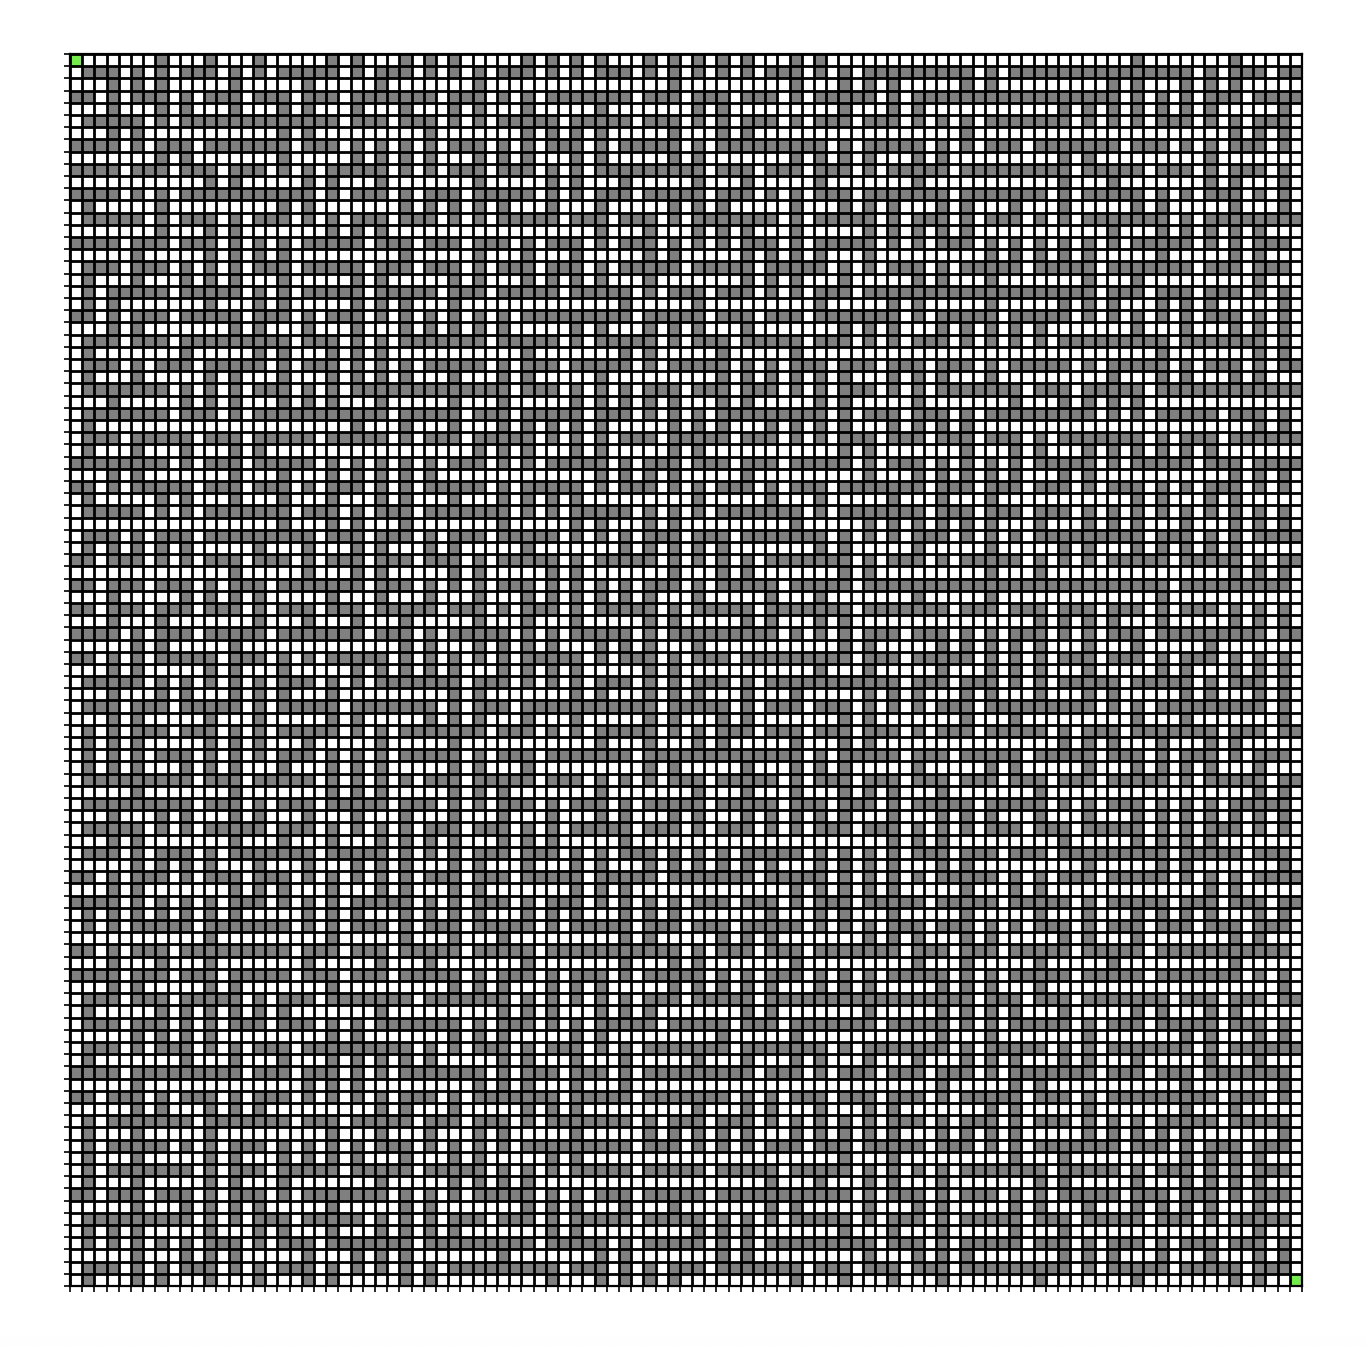
\includegraphics[width=10cm, height=10cm]{empty}
\caption[margin=0.1cm]{Visualization of empty 101 x 101 grid}
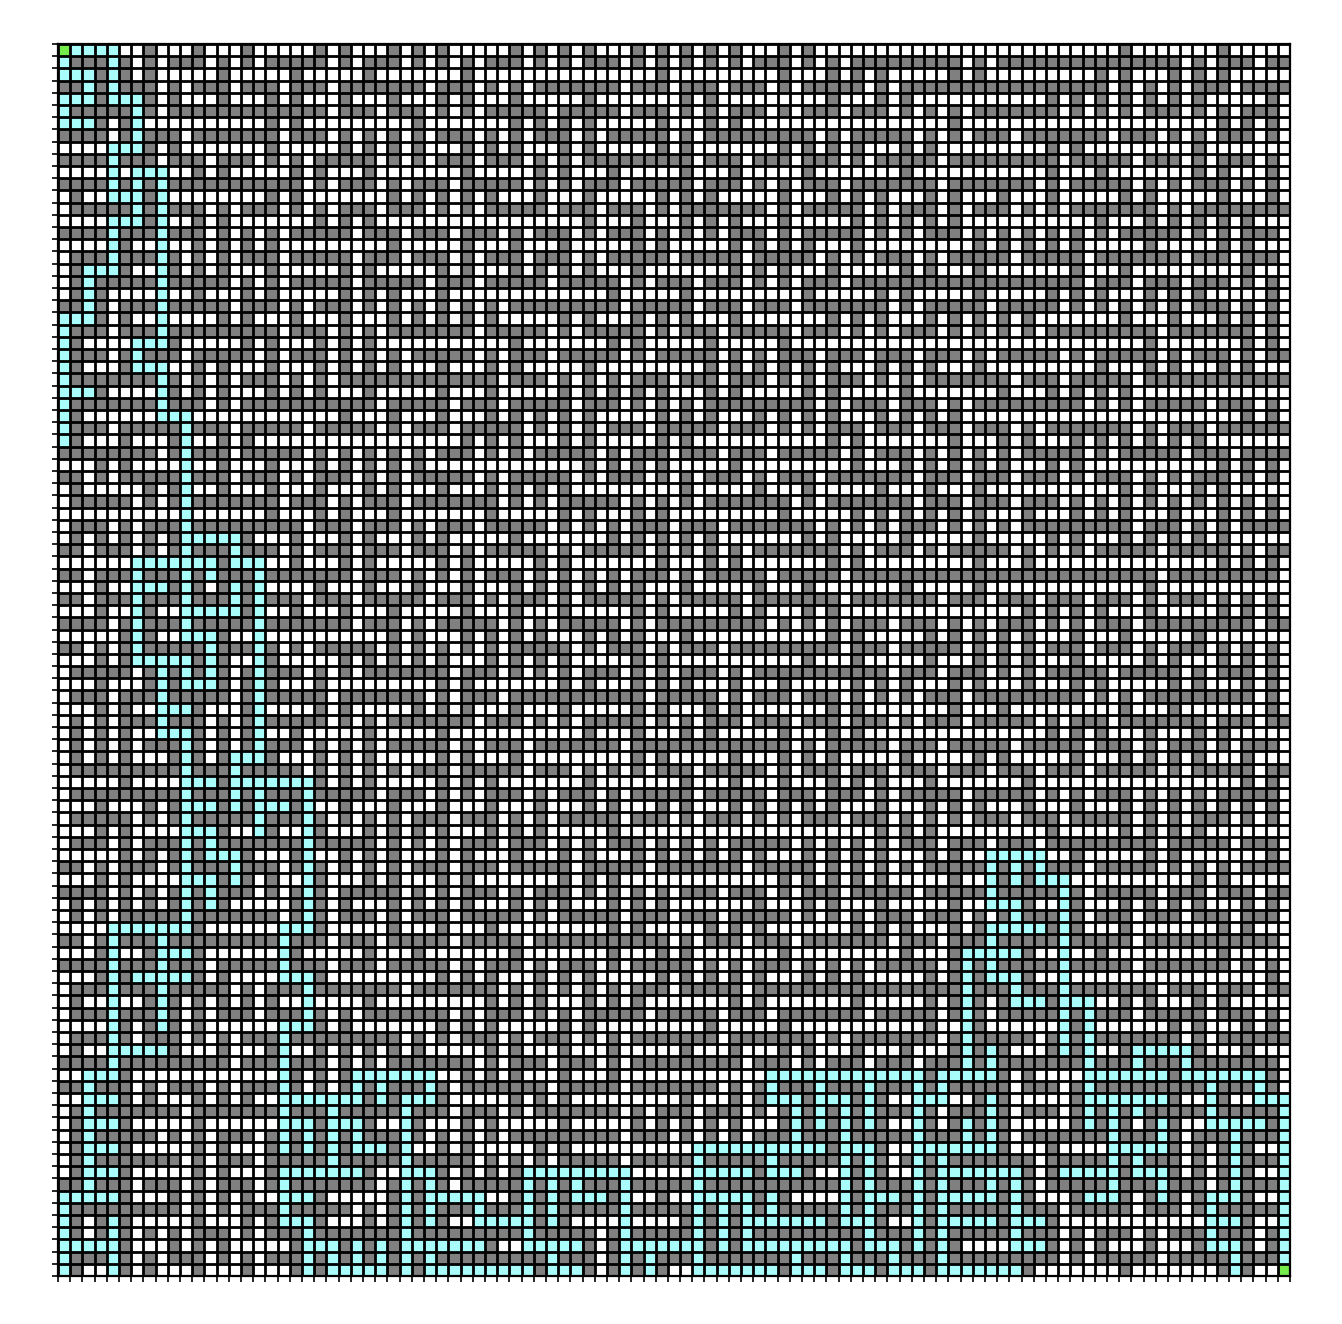
\includegraphics[width=10cm, height=10cm]{forward}
\caption{Visualization of path traversed by agent after calling Repeated Forward A* on previously generated grid}

\end{figure}
\pagebreak
\section*{Part 1}
a) The reason why the agent will move east rather than north is because the agent does not know about any of the blocked cells that exist during the first execution of forward A*. After expanding the initial cell, our algorithm will compute the heuristic values for neighboring cells E3, E1, and D2. These cells will be stored in the open list, where the cell with the minimum f-value will be expanded. In this case, that is cell E3, since it is closest to the goal cell in terms of having the lowest Manhattan Distance. Since we have no knowledge of obstacles, this process will repeat in the same fashion until we generate the following path: E2 (initial) -> E3 -> E4 -> E5 (goal). 
\\\\
b) Every call of A* generates a shortest path from the current cell to the goal cell given our knowledge of obstacles at the time of the call. After each call, we move forward towards the goal until we either arrive at the goal or are stopped by an obstacle along the path. If we hit an obstacle, the algorithm will keep the presence of this obstacle in mind for the next time it is called. So our next call will generate a new path taking into account that we must avoid the obstacle that we just encountered as well as all previously encountered obstacles. By this logic, through repeated calls of A*, we will be able to find a path to the goal if it exists. If the goal is blocked off by obstacles, then our algorithm will fail to generate a path.
\\
Also, in the worst cast, we can assume that we will call A* from each unblocked cell. We will not call it from the same unlocked cell twice because once we arrive at that cell, we have knowledge of all obstacles directly surrounding it and can plan accordingly to avoid them. We can also assume that in the worst case, each call of A* will require the agent to move across all unblocked cells. In reality, it will be less than this because our open list will prioritize cells with better f-values and our closed list will prevent traversal of the same cell multiple times in one call, but it is safe to assume this as an upper bound. By this logic, we can reason that the total number of moves performed by the agent will be bounded by the number of unblocked cells squared. It is worth noting that in practice, the number of moves will be less, and this is only supposed to serve as an upper bound. 
\pagebreak
\section*{Part 2}
After using both larger and smaller g-values for breaking ties in Repeated Forward A*, we observed that using larger g-values was much faster and required far fewer cells to be expanded in comparison to using smaller g-values. We believe that one possible explanation for this is that we encounter many cells with low g-values near the start of the algorithm. If we prioritize low g-values, we will branch off into exploring a lot of these paths, which will lead to far more paths being explored concurrently. If we prioritize larger g-values instead, we will be more committed to sticking onto one path, which will drastically reduce the branching factor of the algorithm, greatly increasing its runtime. 

\begin{figure}[h!]
\centering
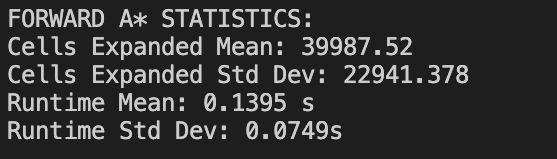
\includegraphics[width=10cm, height=3cm]{forwardstat}
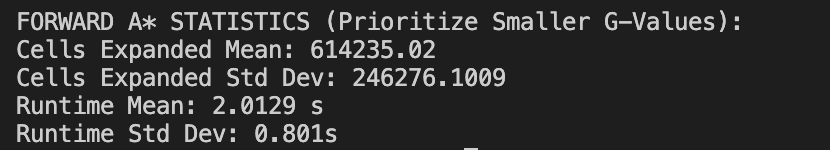
\includegraphics[width=15cm, height=3cm]{smallerg}
\caption[margin=0.1cm]{Larger g-value Statistic vs. Smaller g-value Statistic}
\end{figure}
\pagebreak
\section*{Part 3}
We implemented Repeated Forward A* and Repeated Backward A* and had them both break ties in f-values by favoring larger g-values, and then had them break further ties by using a randomly generated float value. We generated 50 different mazes and tested both algorithms on each maze and compiled the results into different statistics to measure runtime and number of cells expanded by each algorithm. In Figure 4 below, we can see that Repeated Forward A* is significantly faster than Repeated Backward A*, taking almost one second less on average and expanding less cells by a factor of nearly 10. We believe that the reason for this difference is due to the branching factor that is associated with each algorithm when it is expanding cells to look for the path. Repeated Forward A* searches for the path from the initial cell to the goal cell and the robot executes the path in the same direction. Repeated Backward A* searches for the path from the goal cell to the initial cell but the robot is actually executing the path from the initial cell to the goal cell. Because the robot is executing the path from the initial cell to the goal cell in both algorithms we will always first learn about the obstacles surrounding the initial cell and then move out towards the goal cell. Because of this Repeated Backward A* has a higher branching factor when generating adjacent nodes since it doesn’t know about the obstacles near the goal cell but by the initial cell. Repeated Backward A* will explore more nodes and if you visualize the path as a tree it will have more depth because you will learn about the obstacles as you go deeper into the tree, whereas for Repeated Forward A* you will learn about the obstacles earlier on in the tree because you are building the path from the initial cell to the goal cell which is the same direction the robot is moving in. In short, the branching factor for Repeated Backward A* is larger than branching factor for Repeated Forward A*, causing it to be much slower.   
\begin{figure}[p]
\centering
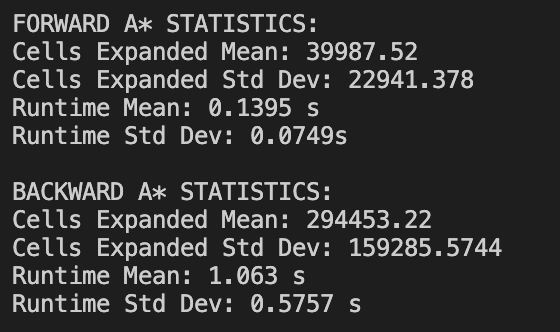
\includegraphics[width=7cm, height=5cm]{fvb_1}
\caption[margin=0.1cm]{Repeated Forward A* Statistics vs Repeated Backward A* Statistics}
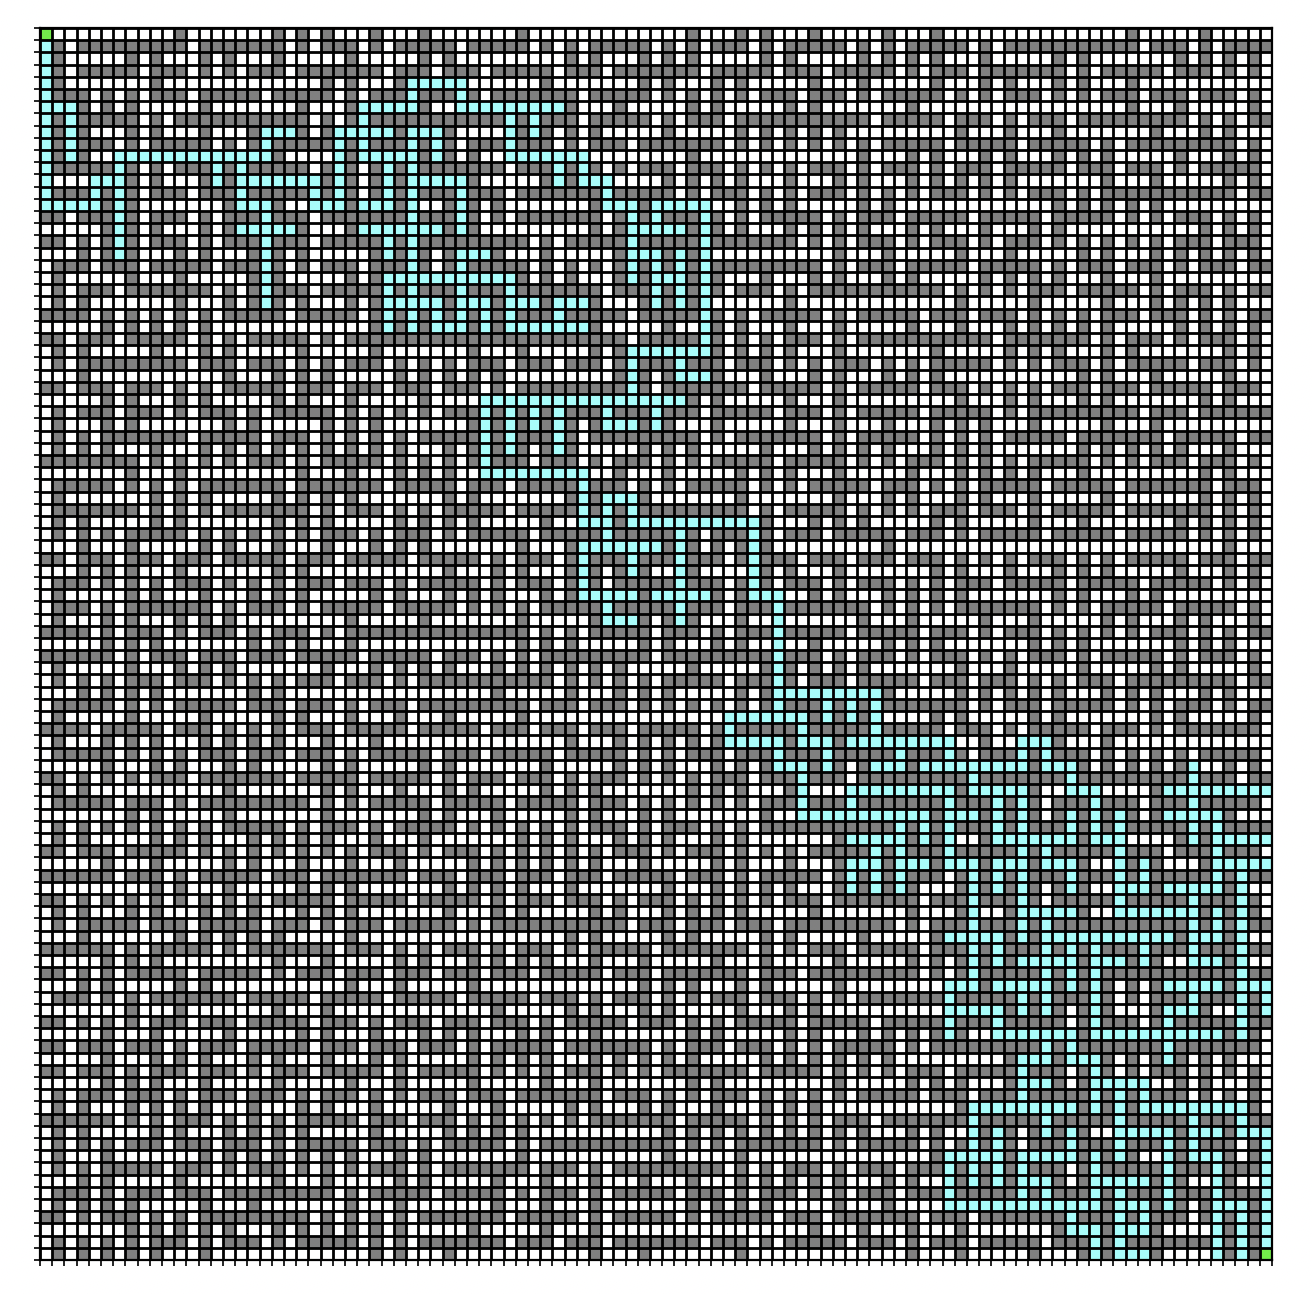
\includegraphics[width=8cm, height=8cm]{forward_b1}
\caption[margin=0.1cm]{Visualization of path traversed by Repeated Forward A* on grid}
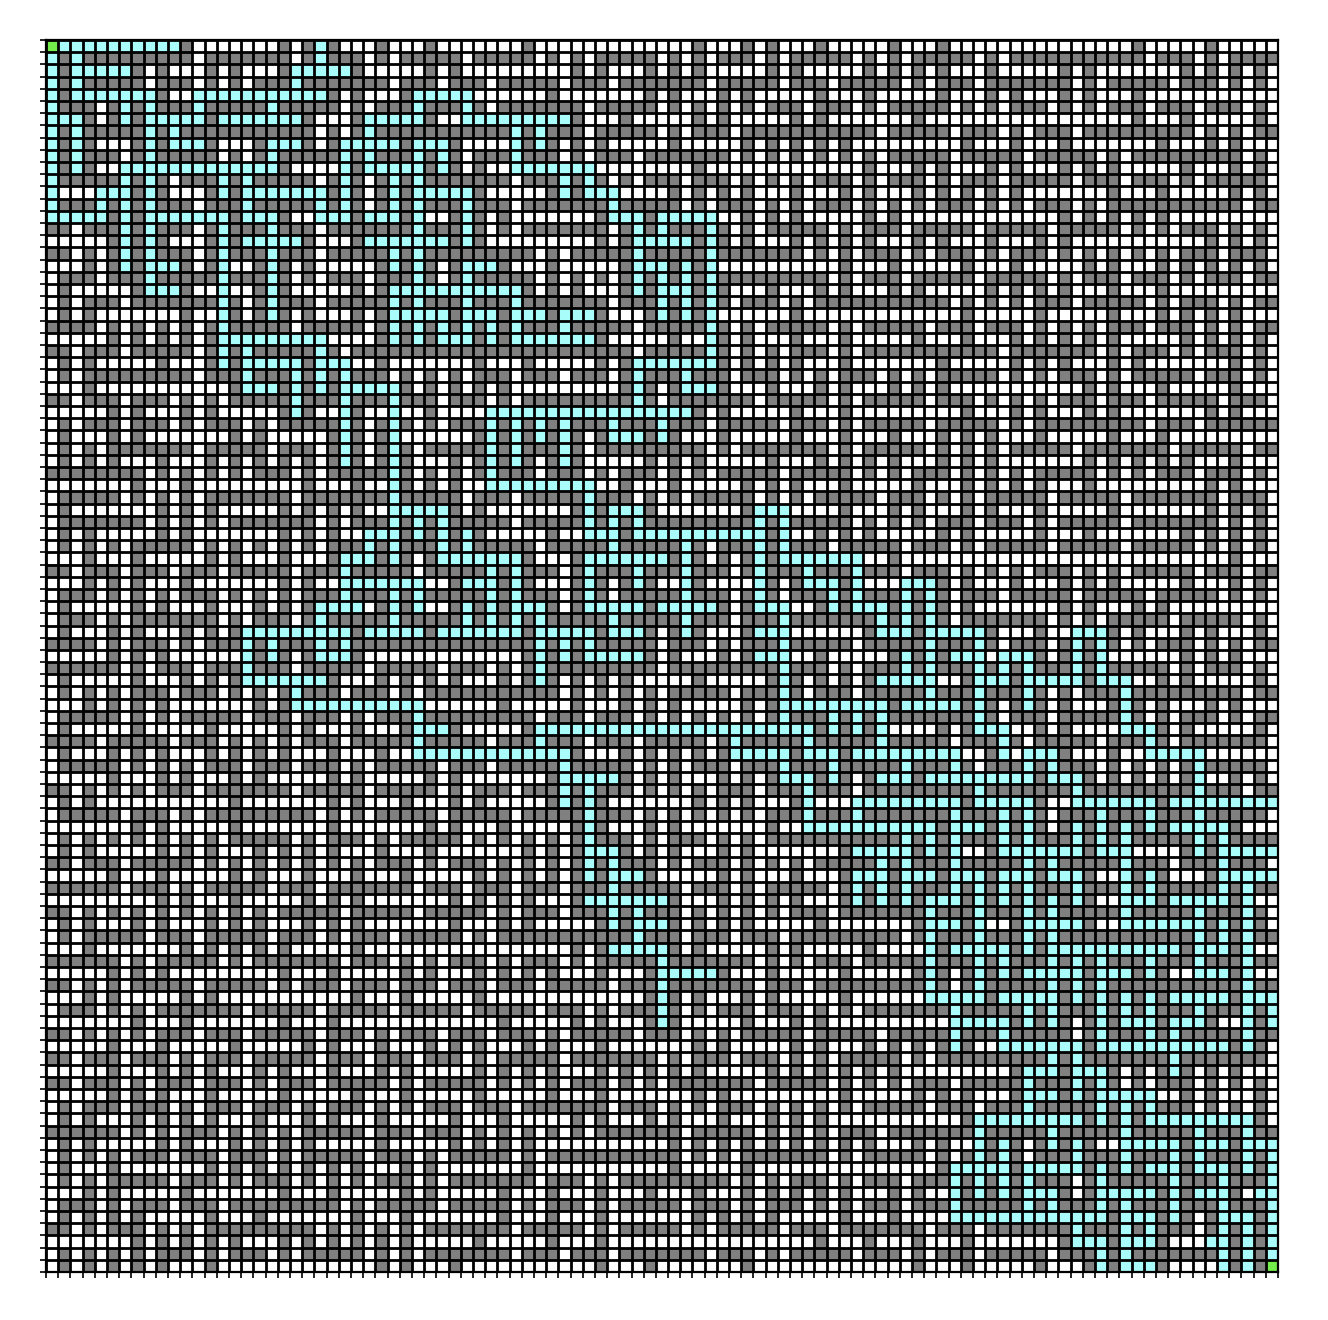
\includegraphics[width=8cm, height=8cm]{f_backward2}
\caption[margin=0.1cm]{Visualization of path traversed by Repeated Backward A* on same grid}
\end{figure}

\pagebreak
\section*{Part 4}
Manhattan distance is defined as the distance from the current cell to any other cell in the maze where distance represents the sum of the magnitudes of the differences between the x and y coordinates of two cells. The robot is able to move repeatedly in any of four directions (up, down, left, or right) to reach the goal state from the initial state. The Manhattan distance doesn’t allow the robot to move in any diagonal direction as by definition that would mean that the agent’s singular move affected both the x and y coordinate, which would either lower or increase the manhattan distance by 2. Manhattan distance can only be consistent with a singular move that will only affect the x or y coordinate, so in one move the Manhattan distance is supposed to only change by 1 with every move. Limiting movement to a single unit up, down, left, and right accomplishes this rule and maintains consistency.
\\~\\
\textbf{Note: The below proofs are based on a traditional 2D Cartesian coordinate system}
\\~\\
Assume \(y_1  > y_0\) and \(x_1 > x_0:\)
\\Start: \((x_0, y_0): h(n) =  (x_1 - x_0) + (y_1 - y_0)\)          
\\Goal: \((x_1, y_1): h(n_{goal}) = 0\)
\\Next Moves:
\\\((x_0, y_0 - 1): 	h(n’) = (x_1 - x_0) + (y_1 - y_0)  + 1\) \quad(down)
\\\((x_0 - 1, y_0): 	h(n’) = (x_1 - x_0) + (y_1 - y_0)  + 1\) \quad(left)
\\\((x_0, y_0 + 1): 	h(n’) = (x_1 - x_0) + (y_1 - y_0)  - 1\)	 \quad(up)
\\\((x_0 + 1, y_0): 	h(n’) = (x_1 - x_0) + (y_1 - y_0)  - 1\)	 \quad(right)
\\
\\\textbf{Proof 1:}
\\Check if triangle inequality holds (assume agent moved one unit up or right from initial cell):
\\
\(h(n) \le c(n, a, n’) + h(n’)\)
\\
\(h(n) \le 1 + h(n) - 1\)
\\
\(h(n) \le h(n)\)
\\
\\\textbf{Proof 2:}
\\Check if triangle inequality holds (assume agent moved one unit down or left from initial cell):
\\
\(h(n) \le c(n, a, n’) + h(n’)\)
\\
\(h(n) \le 1 + h(n) + 1\)
\\
\(h(n) \le h(n) + 2\)
\\
\\The last lines of both proofs above hold true. Moves towards the goal decrease the heuristic value by one and come with an action cost of one, while moves away from the goal increase the heuristic value by one and also come with an action cost of one. In both cases, the heuristic will always be consistent.
\\~\\
\textbf{Now, let us argue that Manhattan distances are not consistent in gridworlds in which the agent can move diagonally:}
\\
\\\textbf{Proof By Contradiction:}
\\Say we apply a diagonal move. Assume a diagonal move will maintain consistency in manhattan distances.
\\
\\Start: \((x_0, y_0): h(n) =  (x_1 - x_0) + (y_1 - y_0)\)
\\Goal: \((x_1, y_1): h(n_{goal}) = 0\)
\\\(y_1  > y_0 \) and \( x_1 > x_0\)
\\~\\
Diagonal move: \((x_0 + 1, y_0 + 1): h(n’) = (x_1 - x_0) + (y_1 - y_0) - 2\)
\\~\\
Given:
\\\(h(n) = (x_1 - x_0) + (y_1 - y_0)\)
\\\(c(n, a, n’) = 1\)
\\~\\
Assume n’ is a move 1 diagonal unit towards the goal: \((x_0 + 1, y_0 + 1)\):
\\\(h(n’) = (x_1 - x_0) + (y_1 - y_0) - 2\)
\\\(h(n’) = h(n) - 2\)
\\~\\
Check if triangle inequality holds:
\\
\(h(n) \le c(n, a, n’) + h(n’)\)
\\
\(h(n) \le 1 + h(n) - 2\)
\\
\(h(n) \le h(n) - 1\)
\\
\\The final line of our proof clearly does not hold. Therefore, we know through contradiction that diagonal moves are not acceptable to maintain consistency in Manhattan distances.
\\~\\
\textbf{Now, let us argue that Adaptive A* which leaves initially consistent h-values consistent even if action costs can increase:}
\\~\\
Repeated Forward A*:
\\
\(h(n) \le c(n, a, n’) + h(n’)\)	
\\If c(n, a, n’) < c’(n, a, n’), then the following holds:
\\
\(h(n) \le c’(n, a, n’) + h(n’)\)
\\Above represents the original h values that are consistent for all (n, a, n’)
\\
\\Similar logic is used in showing Adaptive A* which leaves initially consistent h-values consistent even if action costs can increase:
\\
\\Given:
\\
\(h(n) \le h_{new}(n)\)
\\
\(h_{new}(n) \le c(n, a, n’) + h_{new}(n’)\)		
\\
\\\textbf{Proof:}
\\If c(n, a, n’) < c’(n, a, n’), then the following holds:
\\
\(h_{new}(n) \le c(n, a, n’) + h_{new}(n’) \le c’(n, a, n’) + h_{new}(n’)\)
\\
\(h_{new}(n) \le c’(n, a, n’) + h_{new}(n’)\)
\\
\\We know from the triangle inequality that \(h(n) \le c(n, a, n’) + h(n’)\) is true for Repeated Forward A* search and Adaptive A* (Given Information). The difference with Adaptive A* is that \(h(n) \le h_{new}(n)\). Once we generate the triangle inequality for Adaptive A*, we must prove that the inequality holds in the case of increasing action costs, or when c(n, a, n’) < c’(n, a, n’). As you can see in the proof, it does hold true.


\pagebreak
\section*{Part 5}
We implemented Repeated Forward A* and Adaptive A* and they both break ties in an identical way. We generated 50 different grids and tested both algorithms on each grid and compiled the results into different statistics to measure runtime and number of cells expanded by each algorithm. From the statistics in Figure 7 below, we observed that Adaptive A* was slightly faster than Repeated Forward A* and the number of cells expanded was also lower. The reason behind this slight difference was due to how the h-values were recomputed in Adaptive A* after each iteration, instead of just sticking with the Manhattan distances. The new h-values took into account the distance between each cell and the goal state according to the actual path computed by the latest call of Forward A*, which provided a slightly more informed cost to use when determining the f-value of the cell. Thus, Adaptive A* had a slight edge over Repeated Forward A* in determining better paths in subsequent calls to the Forward A* algorithm. 
\begin{figure}[p]
\centering
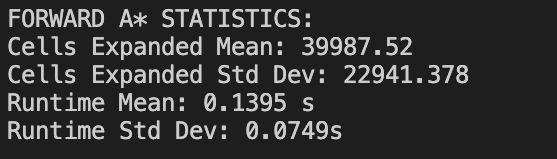
\includegraphics[width=8cm, height=2.5cm]{forwardstat}
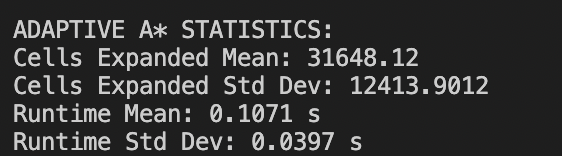
\includegraphics[width=8cm, height=2.5cm]{adaptivestat}
\caption[margin=0.1cm]{Repeated Forward A* Statistics vs. Adaptive A* Statistics}

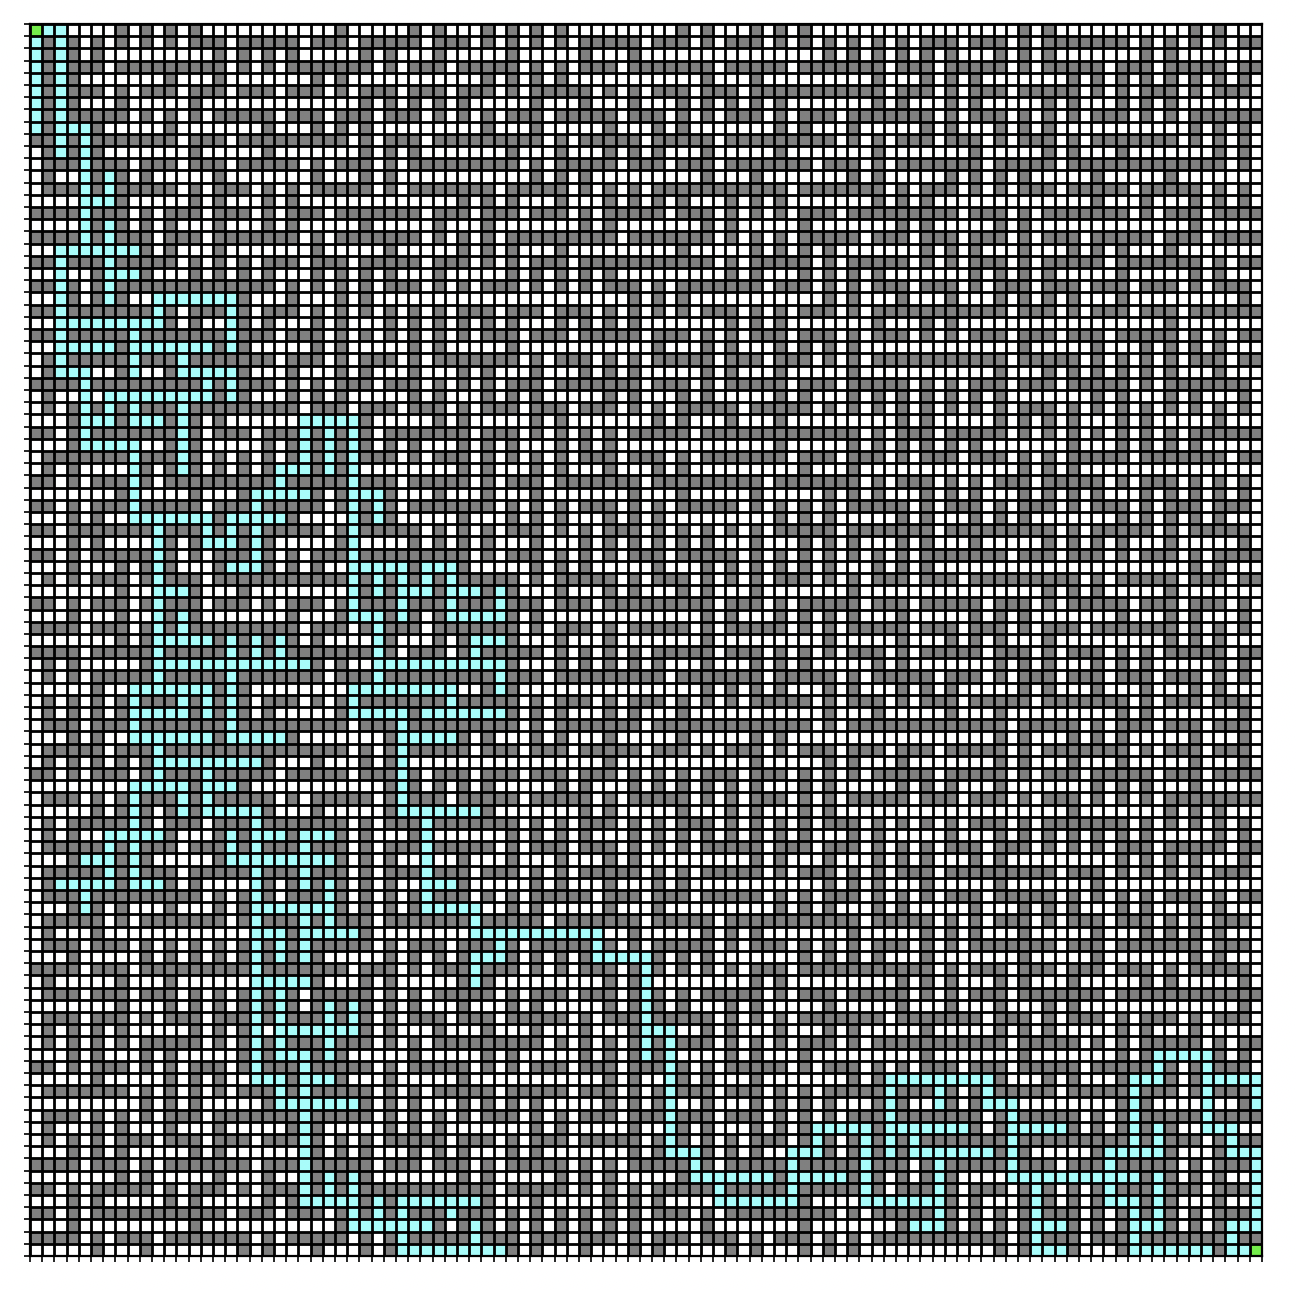
\includegraphics[width=8cm, height=8cm]{forward_a1}
\caption[margin=0.1cm]{Visualization of path traversed by Repeated Forward A* on grid}
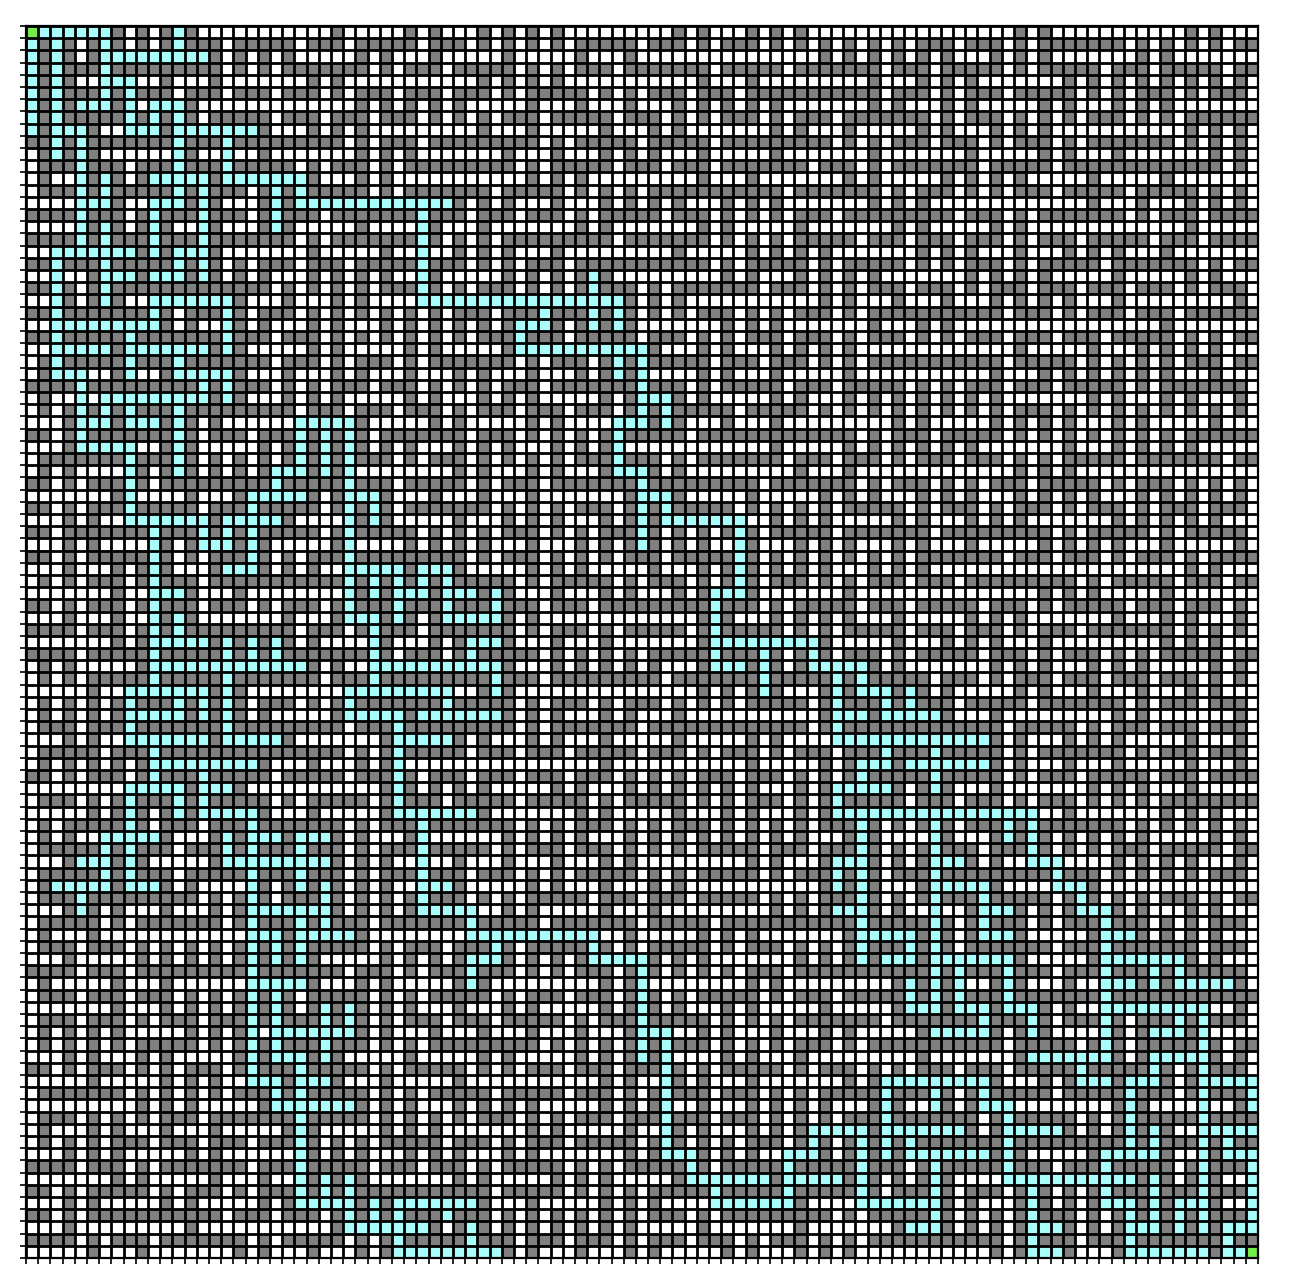
\includegraphics[width=8cm, height=8cm]{f_adaptive2}
\caption[margin=0.1cm]{Visualization of path traversed by Adaptive A* on same grid}

\end{figure}
\pagebreak
\section*{Part 6}
There are multiple steps that can be taken in order to perform a statistical hypothesis test on whether the search algorithms are indeed systematic in nature. For example, we can perform a statistical hypothesis test for number 5 where we looking at the difference in runtimes and number of cells expanded for Repeated Forward A* vs. Adaptive A* or for number 3 where we compare the runtime and number of cells expanded for Repeated Forward A* vs. Repeated Backward A*.
\\~\\
First we make a hypothesis/claim comparing two search algorithms with respect to their runtimes. We can use Null Hypothesis $(H_0)$ and Alternative Hypothesis $(H_1)$ to represent our claims. Alternative Hypothesis is what we are trying to prove and Null Hypothesis is the inverse of it and essentially we reject the Null Hypothesis if the Alternative Hypothesis is true within some probability. Then we design the experiment using independent and dependent variables. Independent variables are variables that are manipulated in the experiment and dependent variables indicate the causal effects of the independent variables.
\\~\\
After designing the experiment, we can run pilot experiments. Pilot experiments test the experiment design and not the hypothesis itself to analyze its validity and make sure if it can actually test the hypothesis or not. Pilot experiments are used to adjust independent and dependent measures. Then we can run the two search algorithms we are comparing across 50 different mazes and compile initial results. From the results we can compile the mean and standard deviation for each search algorithm for comparison. We must do exploratory data analysis to look for reasons behind the results. Since the mean is very sensitive to outliers, it can affect our results, so we can also compile the medians and the frequency distribution to understand the statistics better. Frequency distribution is the frequencies with which the values in a distribution occur and median is the middle value in the data set. Another common concern during these experiments is variance. We always wonder why runtimes and the number of cells expanded are varying so much if the search algorithm is the same. If we care more about the runtimes of the algorithms and less about the problems then we can transform the runtime so the problem has less influence or impact on the runtime and this is known as variance-reducing transformation. 
\\~\\
After obtaining the dataset, we can compute the test statistic which is used to measure the difference between the means that are in the sample data set relative to the variance in the samples. We also compute the probability p or the p-value that corresponds to the test statistic which represents the probability of obtaining the test statistic if the difference between the means were truly 0. The p-value basically is the probability of incorrectly rejecting $H_0$. If the probability or p-value is less than a certain amount known as the level of significance which is defined along with the hypothesis moreover, the probability is very low, then we reject the null hypothesis and we have proven our claim. 
\\~\\
We referred to the following source for information about statistical hypothesis tests: \\\url{http://www.eecs.harvard.edu/cs286r/courses/spring08/reading6/CohenTutorial.pdf}
\end{document}